\documentclass[journal]{IEEEtran}
\usepackage[T1]{fontenc}
\usepackage[utf8]{inputenc}
\usepackage[spanish]{babel}
\usepackage{lmodern}
\usepackage{graphicx}
\usepackage{amsmath}
\usepackage{cite}
\usepackage{listings}
\usepackage{float}
\usepackage{placeins}

\lstset{basicstyle=\ttfamily\footnotesize,columns=flexible,breaklines=true}

\title{Estimación del tiempo de entrega en Olist}

\author{
  \IEEEauthorblockN{Kenneth Eduardo Barboza Corrales\IEEEauthorrefmark{1} \and David Alberto Guevara Sánchez\IEEEauthorrefmark{1}}\\
  \IEEEauthorblockA{\IEEEauthorrefmark{1}Maestría en Ciencias de la Computación, Tecnológico de Costa Rica}
}

\begin{document}

\maketitle

\begin{abstract}
	Se estudió el dataset público de \textit{e-commerce} Olist\cite{olist_dataset} para predecir cuántos días tarda en entregarse cada orden. Se construyó un conjunto de datos unificado con montos de compra, costo de envío, peso, volumen, cantidad de ítems, coordenadas y variables temporales, calculando la distancia geodésica entre cliente y vendedor. Se evitó fuga temporal con un corte cronológico 80/20 (train\_val/test) y validación tomada del 15\% más reciente de train\_val. Como línea base se usó Random Forest y se comparó con XGBoost, LightGBM\cite{ke2017lightgbm} y CatBoost\cite{prokhorenkova2018catboost}. Los mejores resultados se obtuvieron con CatBoost sin tuning (MAE = 4.247 días, RMSE = 5.713), seguido de LightGBM (MAE = 4.294). La distancia fue el predictor más fuerte y los estados del norte presentaron entregas hasta 3 veces más lentas que el sudeste. Los intentos de ajuste de hiperparámetros empeoraron los modelos, por lo que se mantuvieron las configuraciones por defecto.
\end{abstract}

\begin{IEEEkeywords}
	aprendizaje automático, logística, comercio electrónico, random forest, gradient boosting, CatBoost
\end{IEEEkeywords}

\section{Introducción}

Calcular el tiempo de entrega de una orden es clave para gestionar expectativas de los clientes de \textit{e-commerce}. Este trabajo aborda la predicción de días de entrega usando el dataset público de Olist\cite{olist_dataset}, que contiene órdenes realizadas en Brasil con información de clientes, vendedores, productos y coordenadas. El objetivo es estimar la cantidad de días entre la compra y la entrega, manteniendo el flujo de trabajo sencillo y reproducible.

\section{Metodología}

\subsection{Datos y construcción del conjunto}

Se consultó la base SQLite provista (versión del dataset de Kaggle) unificando órdenes, ítems, clientes, vendedores y datos geográficos. Se filtraron únicamente órdenes entregadas con información completa y se agregaron todas las filas por orden, obteniendo un conjunto final de 95{,}978 órdenes con 22 atributos. Las características clave incluyen:
\begin{itemize}
	\item Totales por orden: precio, costo de envío, peso, volumen y número de ítems.
	\item Coordenadas promedio por código postal de cliente y vendedor; para órdenes con varios vendedores se promedió su ubicación.
	\item Distancia geodésica cliente-vendedor en kilómetros.
	\item Variables temporales de compra (mes, día de semana, hora) y categorías auxiliares (fin de semana, horario laboral, indicador de mismo estado y de región remota).
	\item Variable objetivo: días efectivos de entrega calculados como diferencia entre la fecha de compra y la fecha de entrega.
\end{itemize}

\subsection{Ingeniería de características}

A partir del análisis exploratorio se derivaron nueve características adicionales para capturar patrones no lineales y regionales:
\begin{enumerate}
	\item \textbf{Categoría de distancia}: discretización en cuatro rangos---local $<100$ km (17{,}852 órdenes), regional $100$--$500$ km (37{,}123), larga distancia $500$--$1000$ km (25{,}678), muy larga $>1000$ km (15{,}302).
	\item \textbf{Mismo estado}: indicador binario cuando cliente y vendedor comparten estado (36\% de las órdenes).
	\item \textbf{Densidad}: cociente peso/volumen (g/cm$^3$), alternativa a incluir ambas variables correlacionadas ($r=0.83$).
	\item \textbf{Precio por ítem}: precio total dividido por cantidad de ítems.
	\item \textbf{Costo de envío por kilómetro}: flete normalizado por distancia más uno.
	\item \textbf{Cliente en región remota}: indicador para estados del norte (RR, AP, AM, AC, RO, PA), que representan 1.6\% de los clientes.
	\item \textbf{Vendedor en región remota}: indicador análogo para vendedores (0.03\%).
	\item \textbf{Compra en fin de semana}: indicador de compras en sábado o domingo (23\%).
	\item \textbf{Compra en horario laboral}: indicador de compras entre 9 y 18 h (62\%).
\end{enumerate}
Las características de región remota y sureste capturan la brecha logística observada entre el norte y el sudeste del país.

\subsection{Partición y preprocesamiento}

Para evitar fuga temporal, los datos se ordenaron por fecha de compra. El 20\% más reciente quedó como \textit{test}; dentro del 80\% restante, el 15\% final se usó como \textit{validación} y el resto como \textit{train}. Las fechas de entrega y sus derivados se excluyeron de las \textit{features} para no introducir información futura.

El preprocesamiento combina variables categóricas y numéricas mediante un \texttt{ColumnTransformer}: las categorías se codifican con \textit{one-hot} y las variables numéricas se dejan sin escalar, pues los modelos de árboles no lo requieren.

La Tabla~\ref{tab:particion} deja trazados los tamaños y rangos de fechas usados en cada conjunto.

\begin{table}[H]
	\centering
	\caption{Partición temporal empleada en el experimento.}
	\label{tab:particion}
	\begin{tabular}{lrr}
		\hline
		Conjunto      & Registros & Rango de compra          \\
		\hline
		Entrenamiento & 65{,}264  & 2016-09-15 -- 2018-04-06 \\
		Validación    & 11{,}518  & 2018-04-06 -- 2018-05-26 \\
		Prueba        & 19{,}196  & 2018-05-26 -- 2018-08-29 \\
		\hline
	\end{tabular}
\end{table}

\subsection{Modelos y métricas}

Se usó MAE como métrica principal y RMSE como complemento. Se entrenaron los modelos en \textit{train}, se midieron en \textit{validación} y se reportaron resultados finales en \textit{test}. Para los ajustes de hiperparámetros se empleó \textit{RandomizedSearchCV} con \textit{TimeSeriesSplit} (3 particiones) y 50 iteraciones por modelo, explorando parámetros como profundidad máxima, tasa de aprendizaje, número de estimadores y regularización. Los modelos probados fueron:
\begin{itemize}
	\item Random Forest (200 árboles) como línea base.
	\item XGBoost baseline y ajuste aleatorio.
	\item LightGBM baseline y ajuste aleatorio\cite{ke2017lightgbm}.
	\item CatBoost baseline y ajuste aleatorio orientado a categorías\cite{prokhorenkova2018catboost}.
\end{itemize}

\subsection{Flujo de trabajo}

La Figura~\ref{fig:pipeline} esquematiza el pipeline completo desde la ingesta hasta la evaluación.

\begin{figure}[H]
	\centering
	\setlength{\fboxsep}{6pt}
	\begin{tabular}{c}
		\fbox{\parbox{0.9\linewidth}{\textbf{Ingesta SQLite}             \\ Unificación de órdenes, ítems, clientes y vendedores con agregados por orden (precio, flete, peso, volumen, ítems)}}\\[8pt]
		$\downarrow$                                                     \\[8pt]
		\fbox{\parbox{0.9\linewidth}{\textbf{Enriquecimiento geográfico} \\ Lat/lon promedio por código postal y distancia geodésica cliente--vendedor}}\\[8pt]
		$\downarrow$                                                     \\[8pt]
		\fbox{\parbox{0.9\linewidth}{\textbf{Partición temporal}         \\ Corte 80/20 (train\_val/test) y 85/15 dentro de train\_val para validación; sin atributos derivados de la fecha de entrega}}\\[8pt]
		$\downarrow$                                                     \\[8pt]
		\fbox{\parbox{0.9\linewidth}{\textbf{Preprocesamiento}           \\ ColumnTransformer con one-hot para categorías y paso directo de numéricos}}\\[8pt]
		$\downarrow$                                                     \\[8pt]
		\fbox{\parbox{0.9\linewidth}{\textbf{Entrenamiento y evaluación} \\ Modelos de árboles (RF, XGBoost, LightGBM, CatBoost) con MAE/RMSE y sesgo en test}}\\
	\end{tabular}
	\caption{Flujo del pipeline de modelado.}
	\label{fig:pipeline}
\end{figure}

\section{Resultados}

\subsection{Exploración de datos}

La variable objetivo tiene mediana 10.2 días y media 12.5, con cola larga de valores atípicos por encima de 30 días. Usando el criterio de 1.5$\times$IQR, se identificaron 4{,}891 valores atípicos (5.1\% del total) por encima del umbral de 29.12 días; el máximo alcanza 209.63 días. La Figura~\ref{fig:distribucion} muestra el histograma y el boxplot: el pico principal se ubica entre 7 y 15 días y aparecen entregas extremas por arriba de 200 días.

\begin{figure}[H]
	\centering
	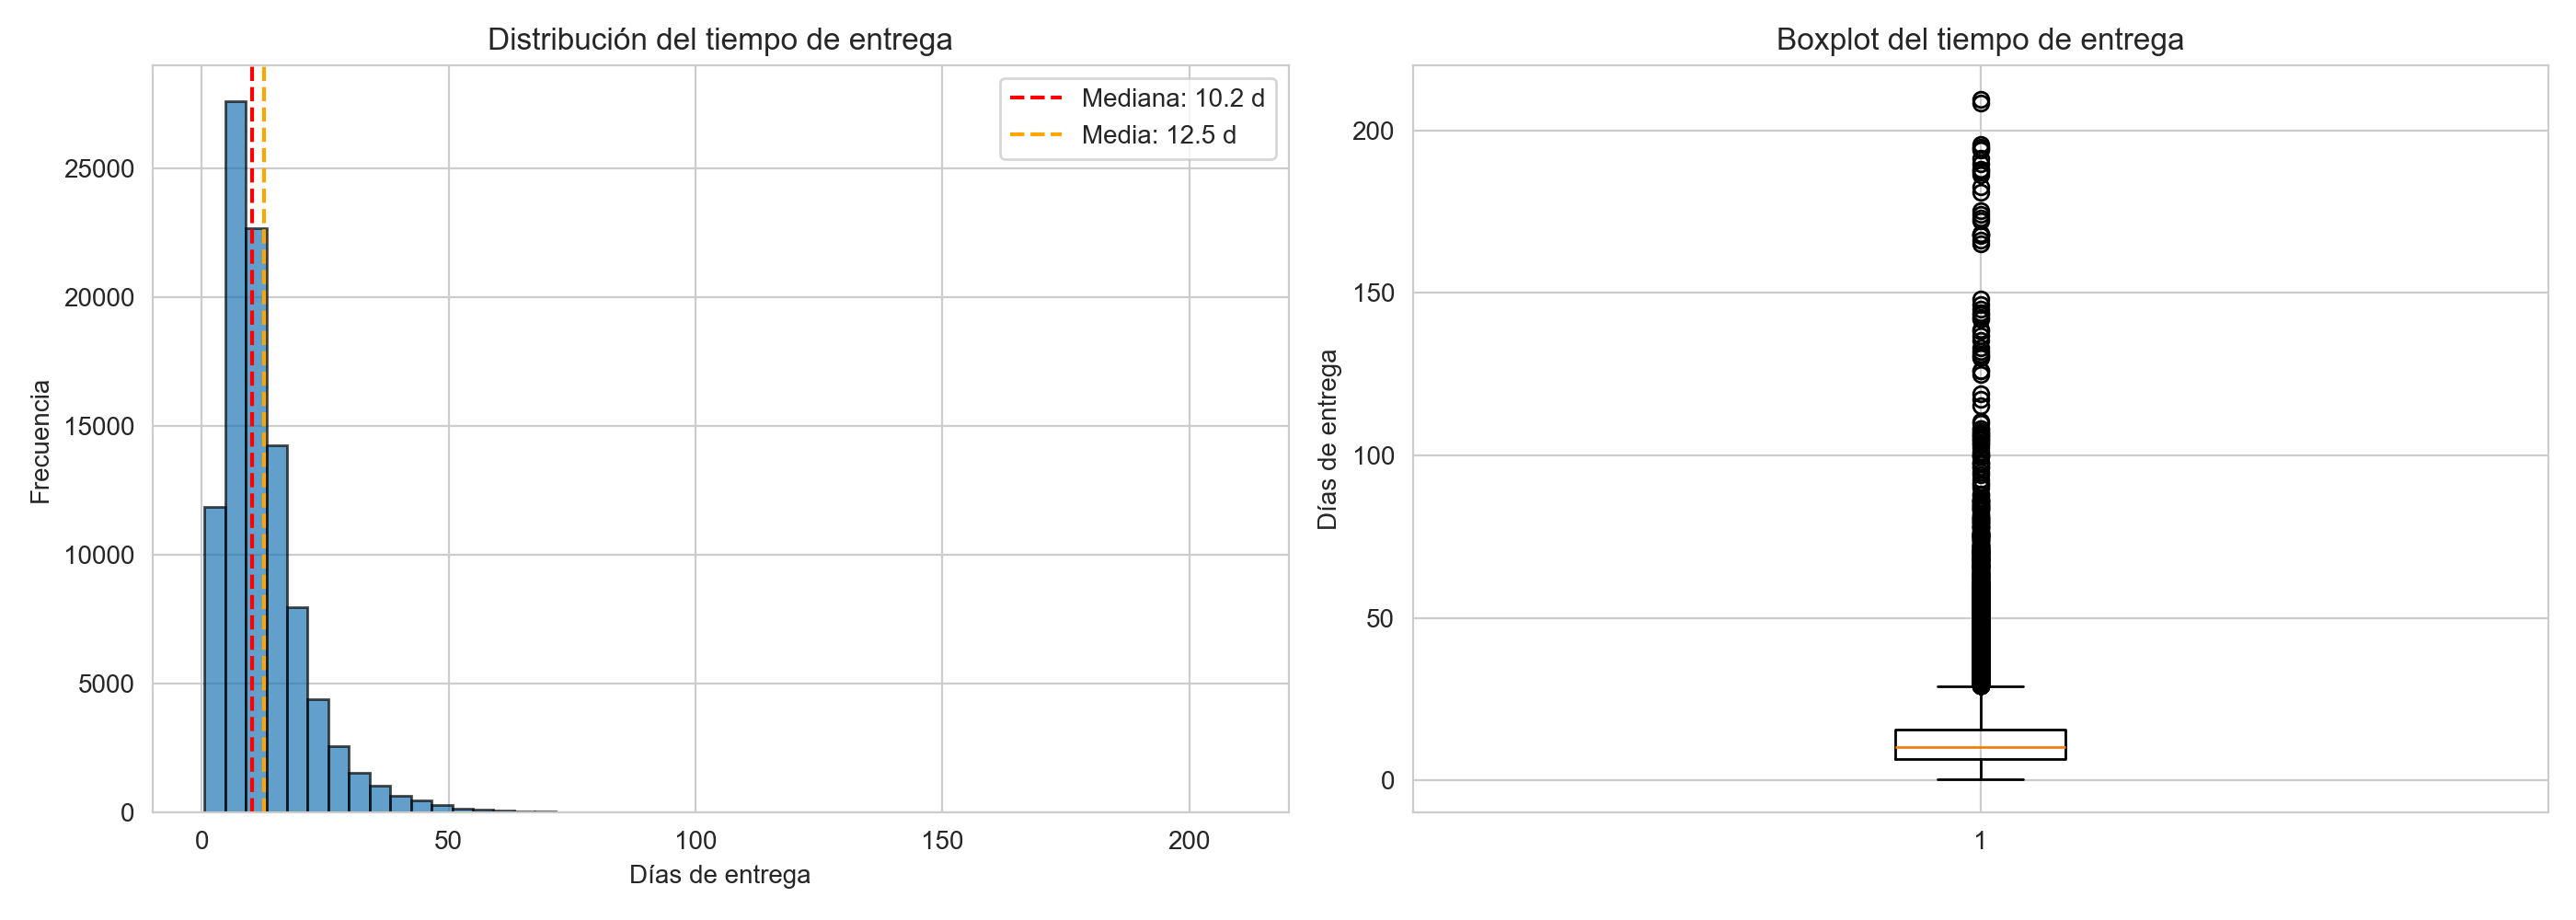
\includegraphics[width=\linewidth]{figures/distribucion_entrega.png}
	\caption{Distribución del tiempo de entrega. Asimetría a la derecha y valores atípicos por encima de 30 días.}
	\label{fig:distribucion}
\end{figure}

Las fechas de compra y entrega presentan estacionalidad: agosto es el mes con más órdenes y septiembre cae abruptamente; en horas, la franja de 15:00 a 20:00 concentra la mayor actividad. Respecto al tiempo de entrega por mes, febrero es el más lento (16.2 días en promedio) y agosto el más rápido (9.1 días), una variación de aproximadamente 7 días entre el peor y el mejor mes. Por hora de compra, las órdenes realizadas a las 4:00 se entregan más rápido que las de medianoche. La Figura~\ref{fig:temporales} resume estos patrones por mes, día de semana y hora para compras y entregas.

\begin{figure}[H]
	\centering
	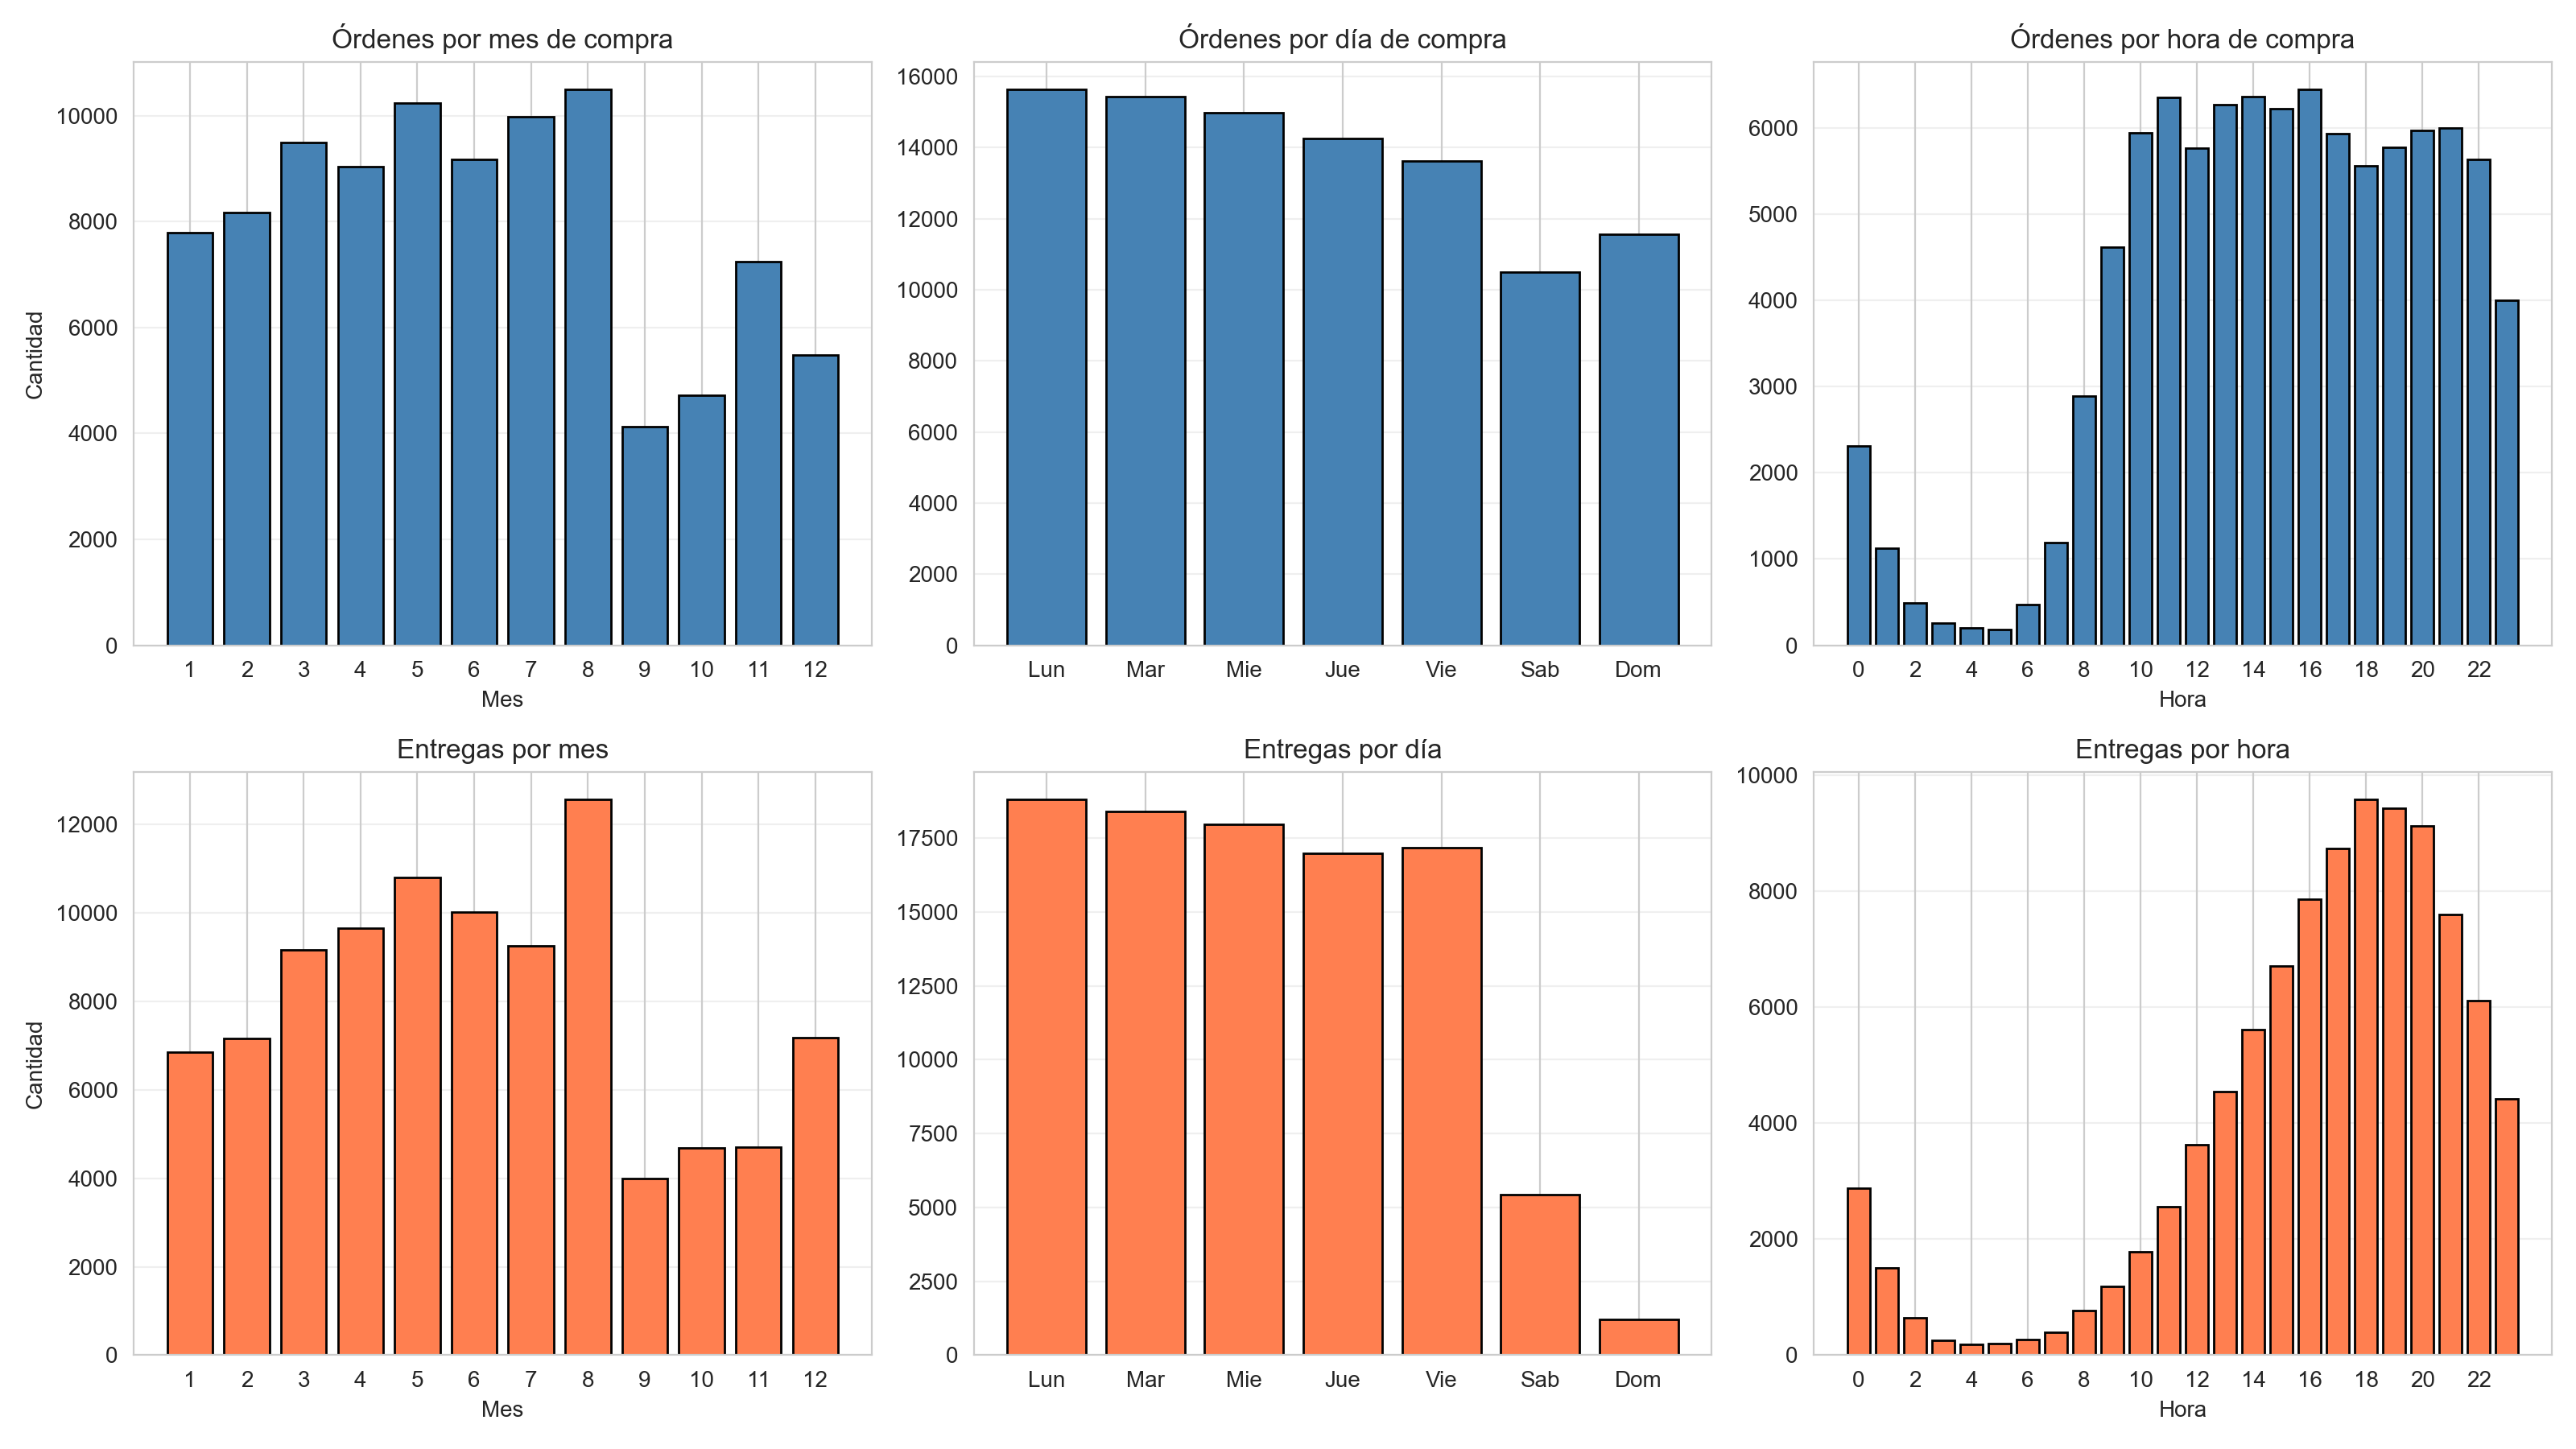
\includegraphics[width=\linewidth]{figures/temporales.png}
	\caption{Patrones temporales de compra (fila superior) y entrega (fila inferior). Agosto es el pico mensual y las 15:00--20:00 son las horas de mayor actividad.}
	\label{fig:temporales}
\end{figure}

La matriz de correlación de la Figura~\ref{fig:correlacion} confirma que la distancia geográfica es el predictor numérico más fuerte del tiempo de entrega ($r=0.394$). El costo de envío correlaciona moderadamente con el tiempo ($r=0.167$), pero se relaciona más con el peso ($r=0.64$) y la distancia ($r=0.315$), indicando que los recargos responden principalmente al tamaño del paquete. Precio total ($r=0.056$) e ítems ($r=-0.019$) tienen correlaciones prácticamente nulas.

\begin{figure}[H]
	\centering
	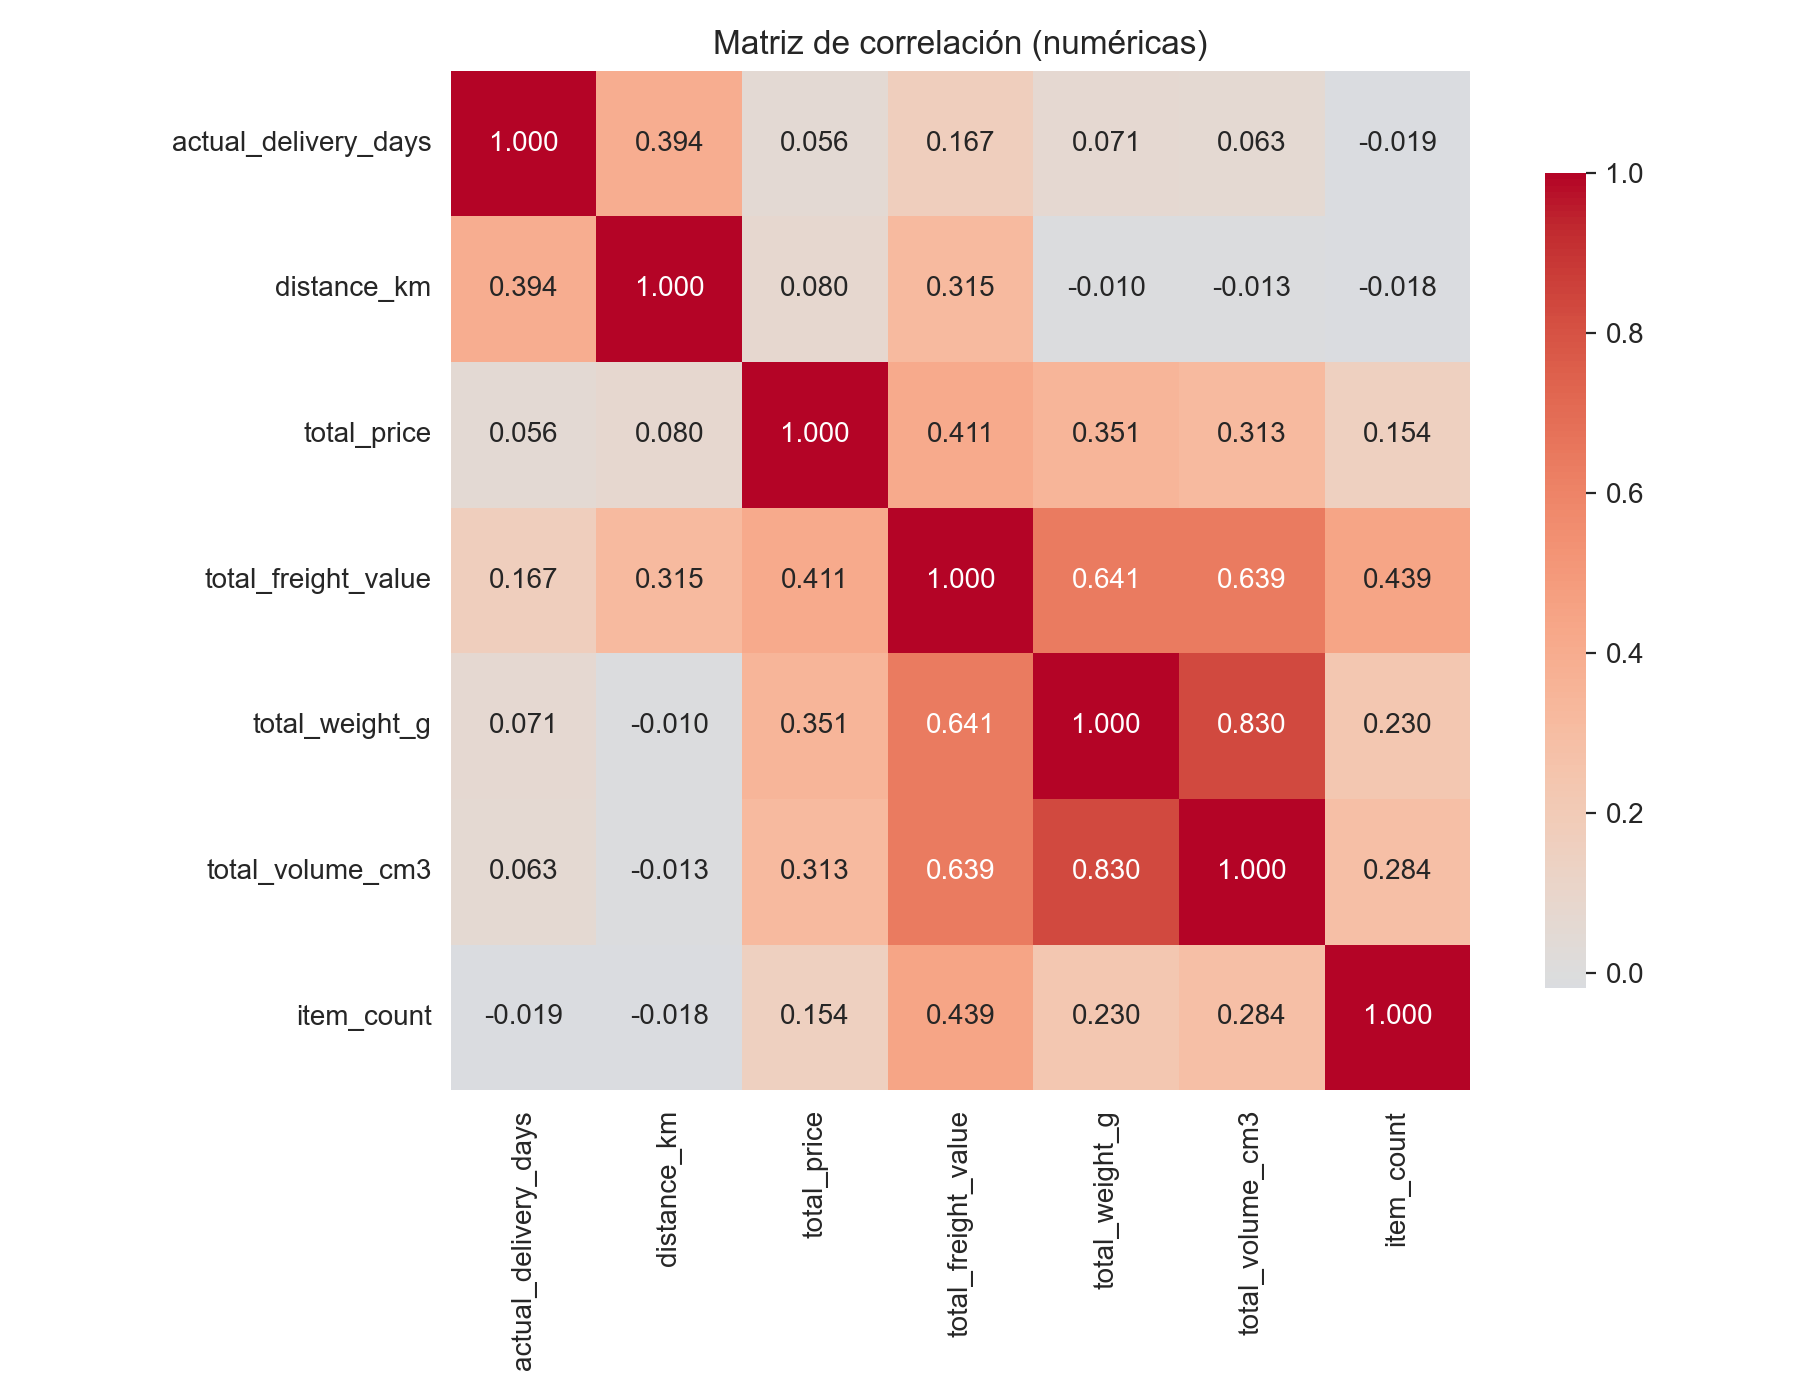
\includegraphics[width=0.9\linewidth]{figures/correlacion.png}
	\caption{Correlación entre variables numéricas. La distancia destaca como la variable más relacionada con los días de entrega.}
	\label{fig:correlacion}
\end{figure}

El dispersograma de la Figura~\ref{fig:distancia} muestra la relación distancia-tiempo. El ajuste lineal ($y = 0.0064x + 8.74$) sugiere un incremento de $\sim$6.4 días por cada 1000 km adicionales, con un tiempo base de 8.7 días incluso para entregas locales. La dispersión vertical es alta: dos órdenes con la misma distancia pueden diferir en $\pm 20$ días.

\begin{figure}[H]
	\centering
	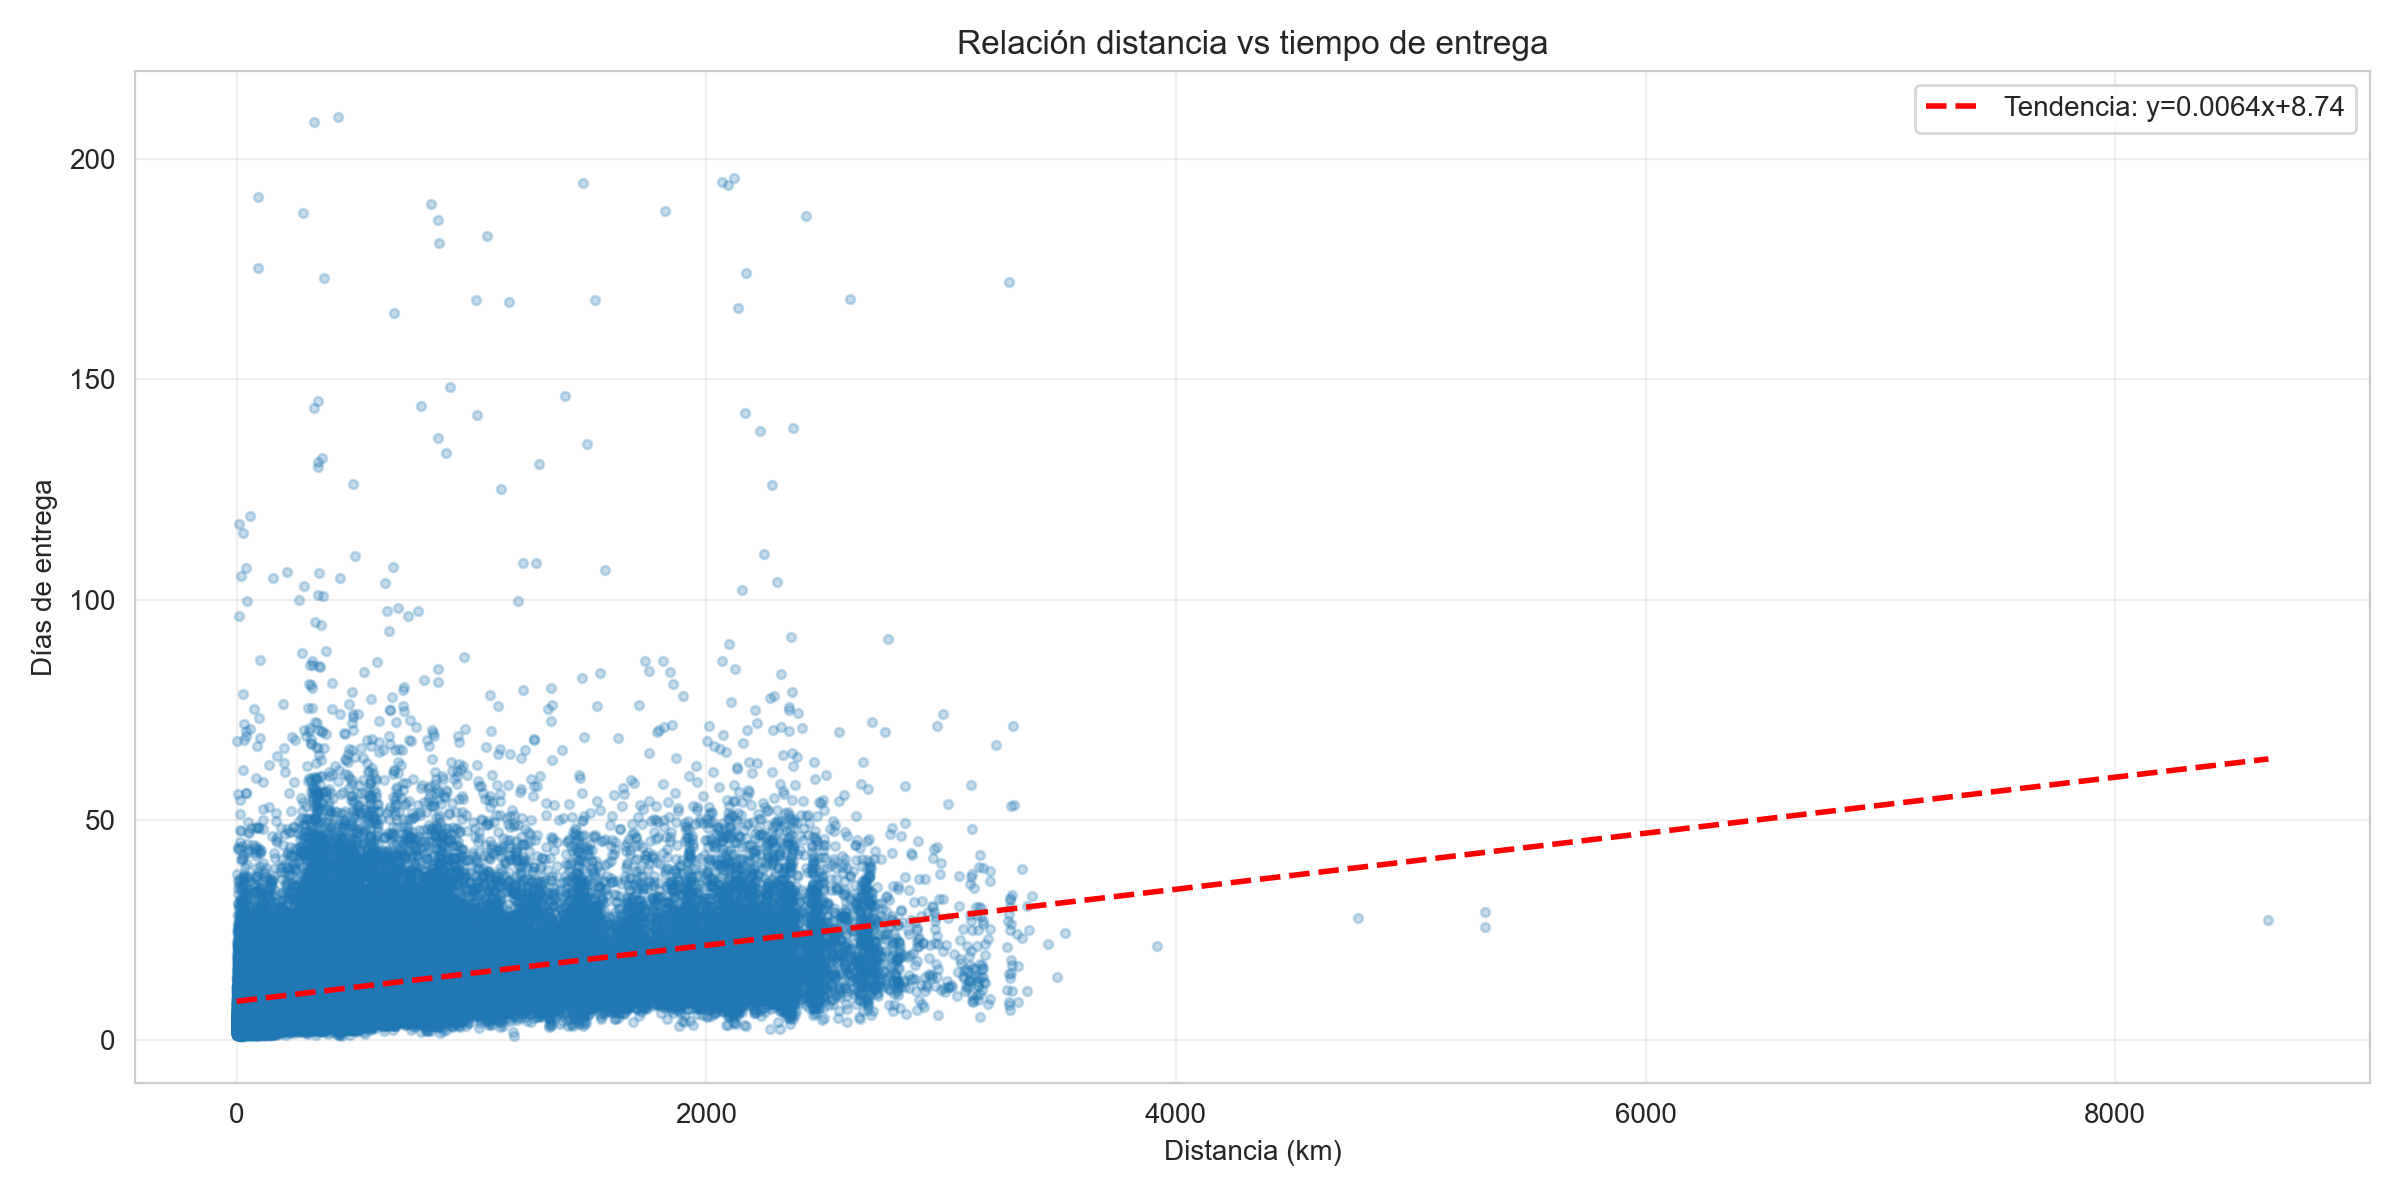
\includegraphics[width=\linewidth]{figures/distancia_vs_tiempo.png}
	\caption{Relación distancia-tiempo. El ajuste lineal estima ~6.4 días extra por 1000 km, con gran dispersión.}
	\label{fig:distancia}
\end{figure}

La Figura~\ref{fig:estado_cliente} detalla el tiempo promedio según el estado del cliente. Los estados remotos del norte (RR, AP, AM) tardan 26--29 días en promedio, mientras que São Paulo entrega en 8.8 días; la brecha supera 3 veces entre regiones.

\begin{figure}[H]
	\centering
	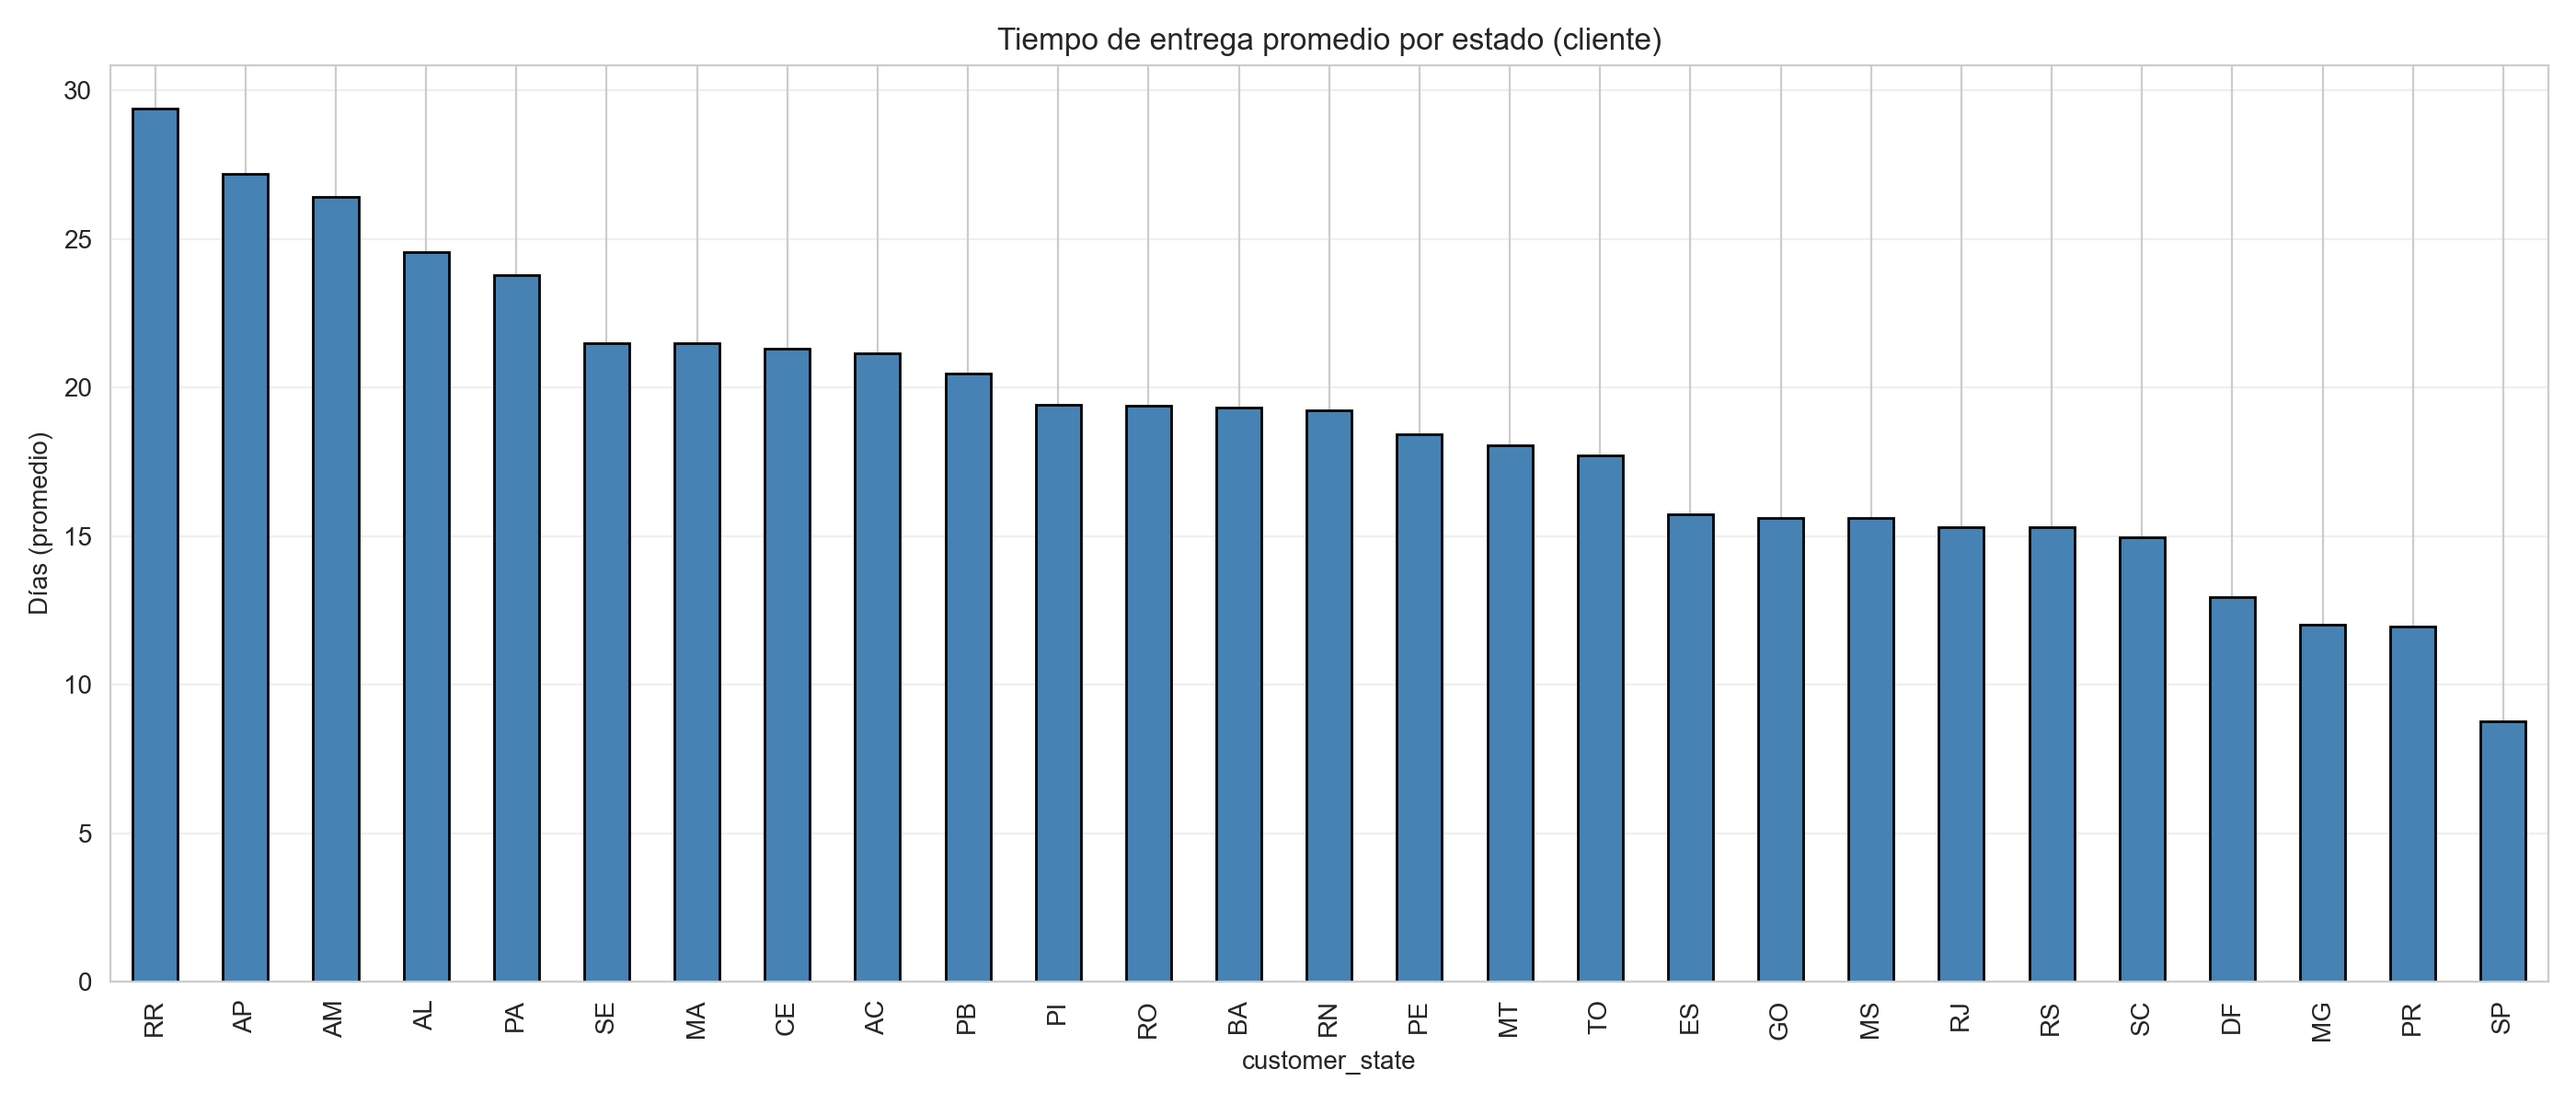
\includegraphics[width=\linewidth]{figures/estado_cliente.png}
	\caption{Promedio de días de entrega por estado del cliente. El norte es el más lento; el sudeste entrega en menos de 15 días.}
	\label{fig:estado_cliente}
\end{figure}

En el rol de vendedor, el panorama es aún más dispar. La Figura~\ref{fig:estado_vendedor} muestra que enviar desde AM lleva en promedio 47.8 días, casi el doble del siguiente estado, mientras la mayoría se ubica entre 11 y 14 días.

\begin{figure}[H]
	\centering
	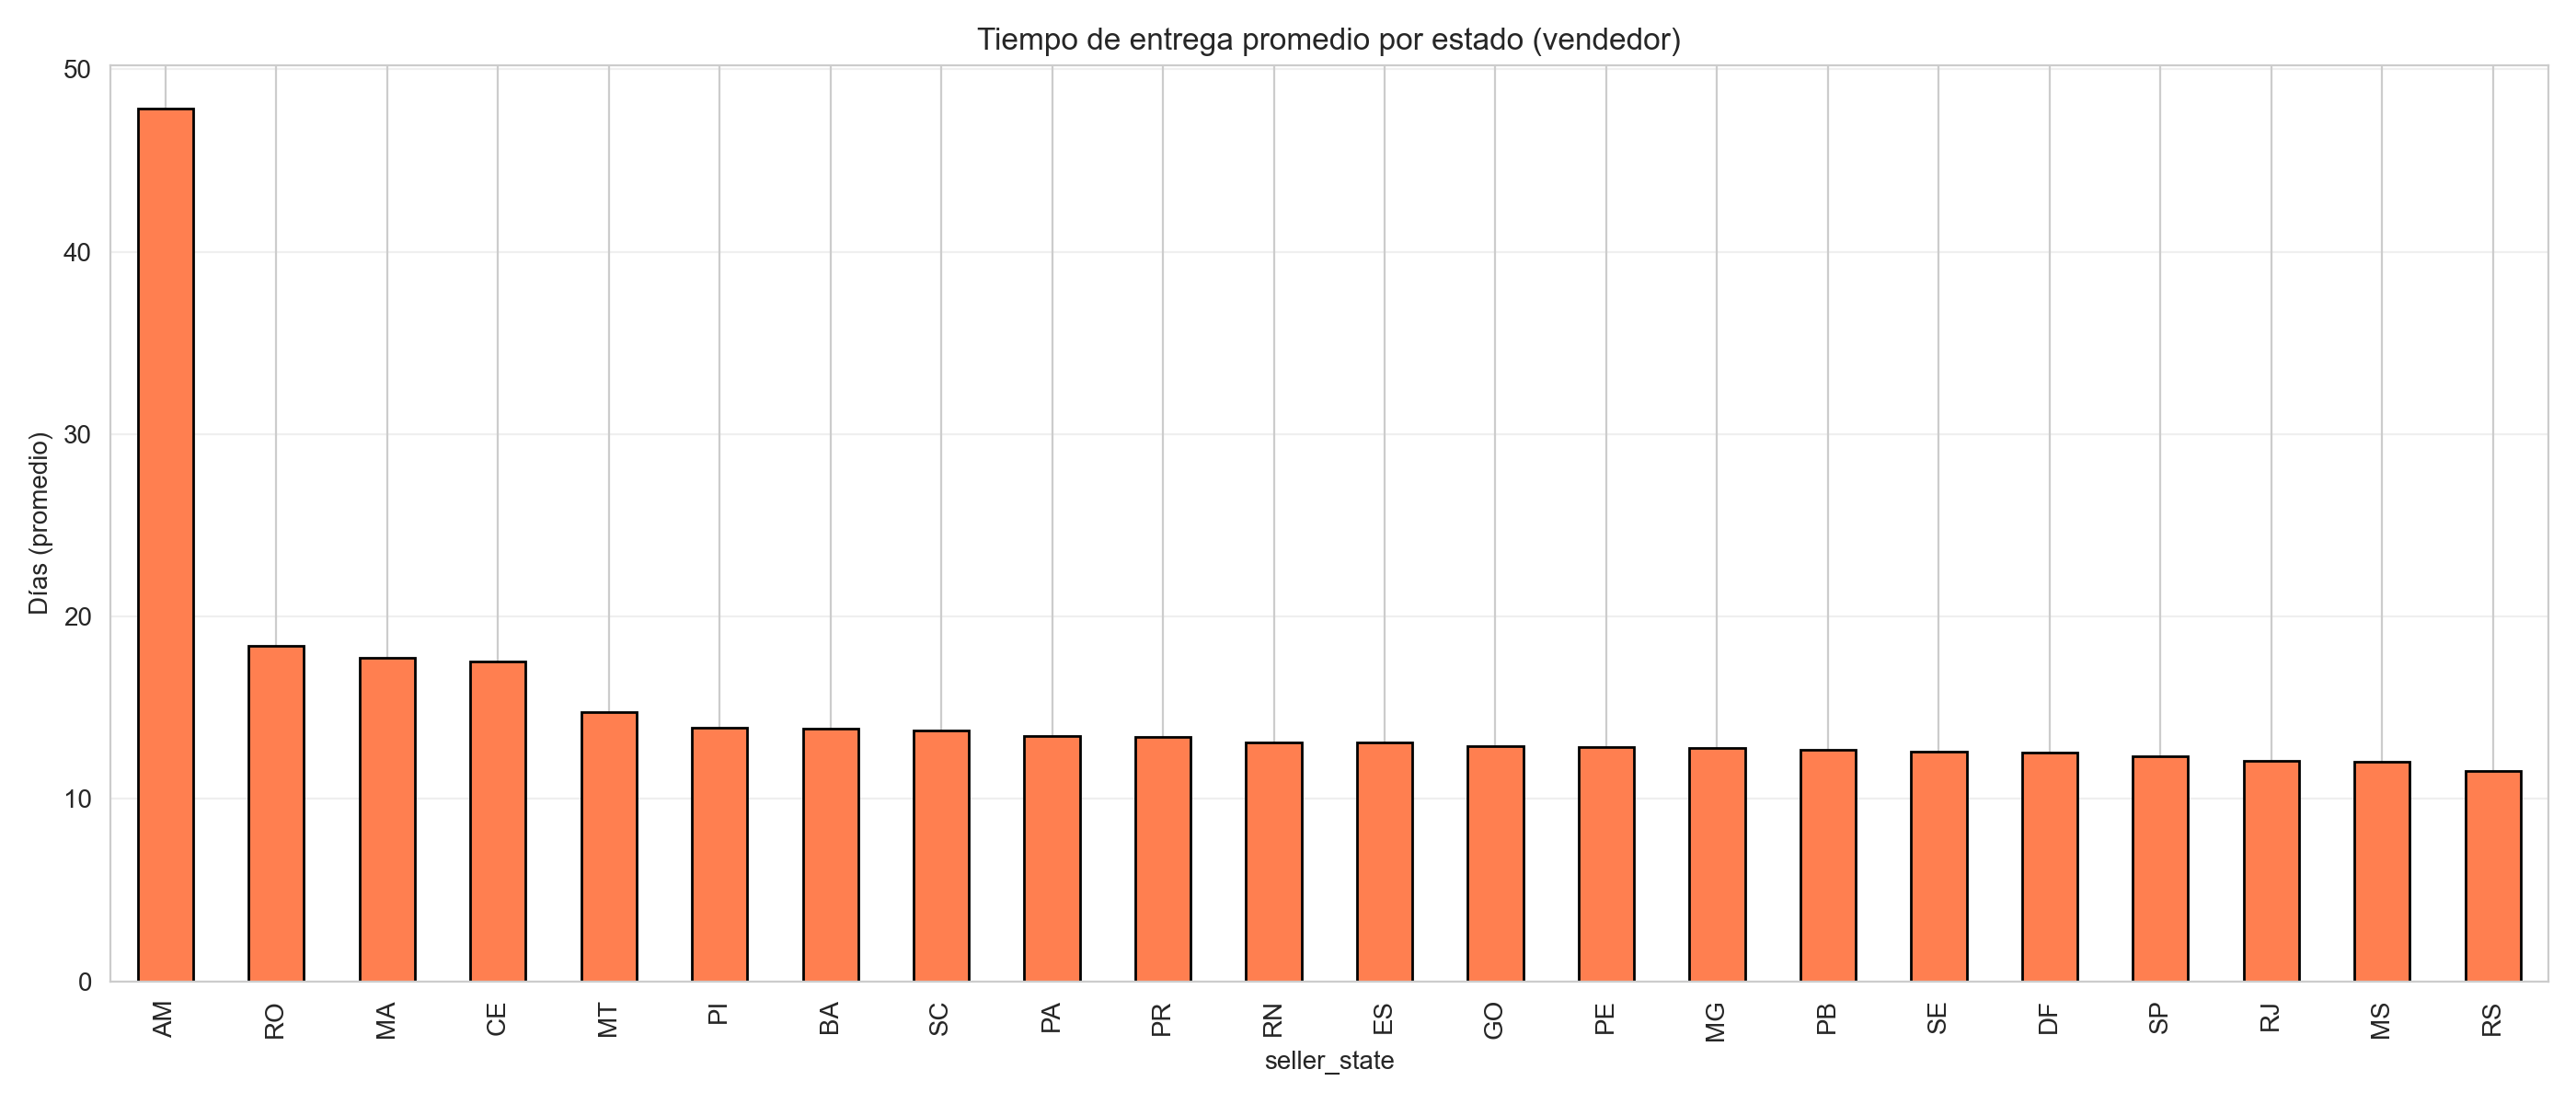
\includegraphics[width=\linewidth]{figures/estado_vendedor.png}
	\caption{Promedio de días de entrega por estado del vendedor. Enviar desde AM es el caso más lento (47.8 días).}
	\label{fig:estado_vendedor}
\end{figure}

\subsection{Comparación de modelos}

La Tabla~\ref{tab:modelos} resume el desempeño en \textit{test} (MAE en días). El Random Forest baseline sirvió como referencia; el ajuste de hiperparámetros lo empeoró (-13.16\%). XGBoost tampoco superó la línea base. LightGBM mejoró 4.07\% y CatBoost fue el mejor con una mejora de 5.11\% sobre Random Forest. Los boosters compartieron un sesgo negativo cercano a -2.4 días, es decir, tienden a sobreestimar ligeramente el tiempo de entrega, lo cual es aceptable para comunicar rangos conservadores.

\begin{table}[H]
	\centering
	\caption{Comparación de modelos en \textit{test} (errores en días).}
	\label{tab:modelos}
	\begin{tabular}{lrr}
		\hline
		Modelo                   & MAE            & RMSE  \\
		\hline
		Random Forest (baseline) & 4.476          & 5.955 \\
		Random Forest (ajustado) & 5.065          & 6.321 \\
		XGBoost (baseline)       & 4.614          & 6.348 \\
		XGBoost (ajustado)       & 4.766          & 5.968 \\
		LightGBM (baseline)      & 4.294          & 5.678 \\
		LightGBM (ajustado)      & 4.321          & 5.705 \\
		CatBoost (baseline)      & \textbf{4.247} & 5.713 \\
		CatBoost (ajustado)      & 4.581          & 5.808 \\
		\hline
	\end{tabular}
\end{table}

Además del MAE, los boosters líderes presentaron RMSE de 5.678 (LightGBM) y 5.713 (CatBoost), confirmando que el error cuadrático sigue la misma tendencia. Respecto al tiempo de entrenamiento, LightGBM baseline se entrenó en apenas 0.85 segundos, mientras que CatBoost requirió 3.77 segundos; las búsquedas aleatorias aumentaron estos tiempos a varios minutos sin compensar el costo adicional con mejoras de desempeño.

La Tabla~\ref{tab:validacion} muestra las métricas en validación, donde los errores fueron mayores que en test debido a la dificultad de las órdenes en ese período. No obstante, el ordenamiento relativo de modelos se mantiene: los boosters LightGBM y CatBoost lideran, y sus variantes ajustadas no superan a las versiones baseline.

\begin{table}[H]
	\centering
	\caption{Métricas en el conjunto de \textit{validación} (errores en días).}
	\label{tab:validacion}
	\begin{tabular}{lrr}
		\hline
		Modelo                   & MAE            & RMSE  \\
		\hline
		Random Forest (baseline) & 4.990          & 7.161 \\
		Random Forest (ajustado) & 4.873          & 6.783 \\
		XGBoost (baseline)       & 5.049          & 7.360 \\
		XGBoost (ajustado)       & 4.933          & 6.876 \\
		LightGBM (baseline)      & 4.699          & 6.739 \\
		LightGBM (ajustado)      & 4.729          & 6.758 \\
		CatBoost (baseline)      & \textbf{4.690} & 6.789 \\
		CatBoost (ajustado)      & 4.917          & 6.891 \\
		\hline
	\end{tabular}
\end{table}

La Tabla~\ref{tab:sesgo} resume el sesgo promedio (error medio) reportado en el cuaderno para los modelos base: todos sobreestiman el tiempo (sesgo negativo), siendo LightGBM y CatBoost los más cercanos a cero.

\begin{table}[H]
	\centering
	\caption{Sesgo promedio (error medio) en \textit{test} para modelos base.}
	\label{tab:sesgo}
	\begin{tabular}{lr}
		\hline
		Modelo                   & Sesgo (días) \\
		\hline
		Random Forest (baseline) & -2.67        \\
		XGBoost (baseline)       & -2.68        \\
		LightGBM (baseline)      & -2.50        \\
		CatBoost (baseline)      & -2.402       \\
		\hline
	\end{tabular}
\end{table}

La Figura~\ref{fig:mae_modelos} ilustra visualmente las diferencias de MAE en \textit{test}: CatBoost baseline encabeza, LightGBM le sigue de cerca y los ajustes aleatorios empeoran sus respectivas líneas base.

\begin{figure}[H]
	\centering
	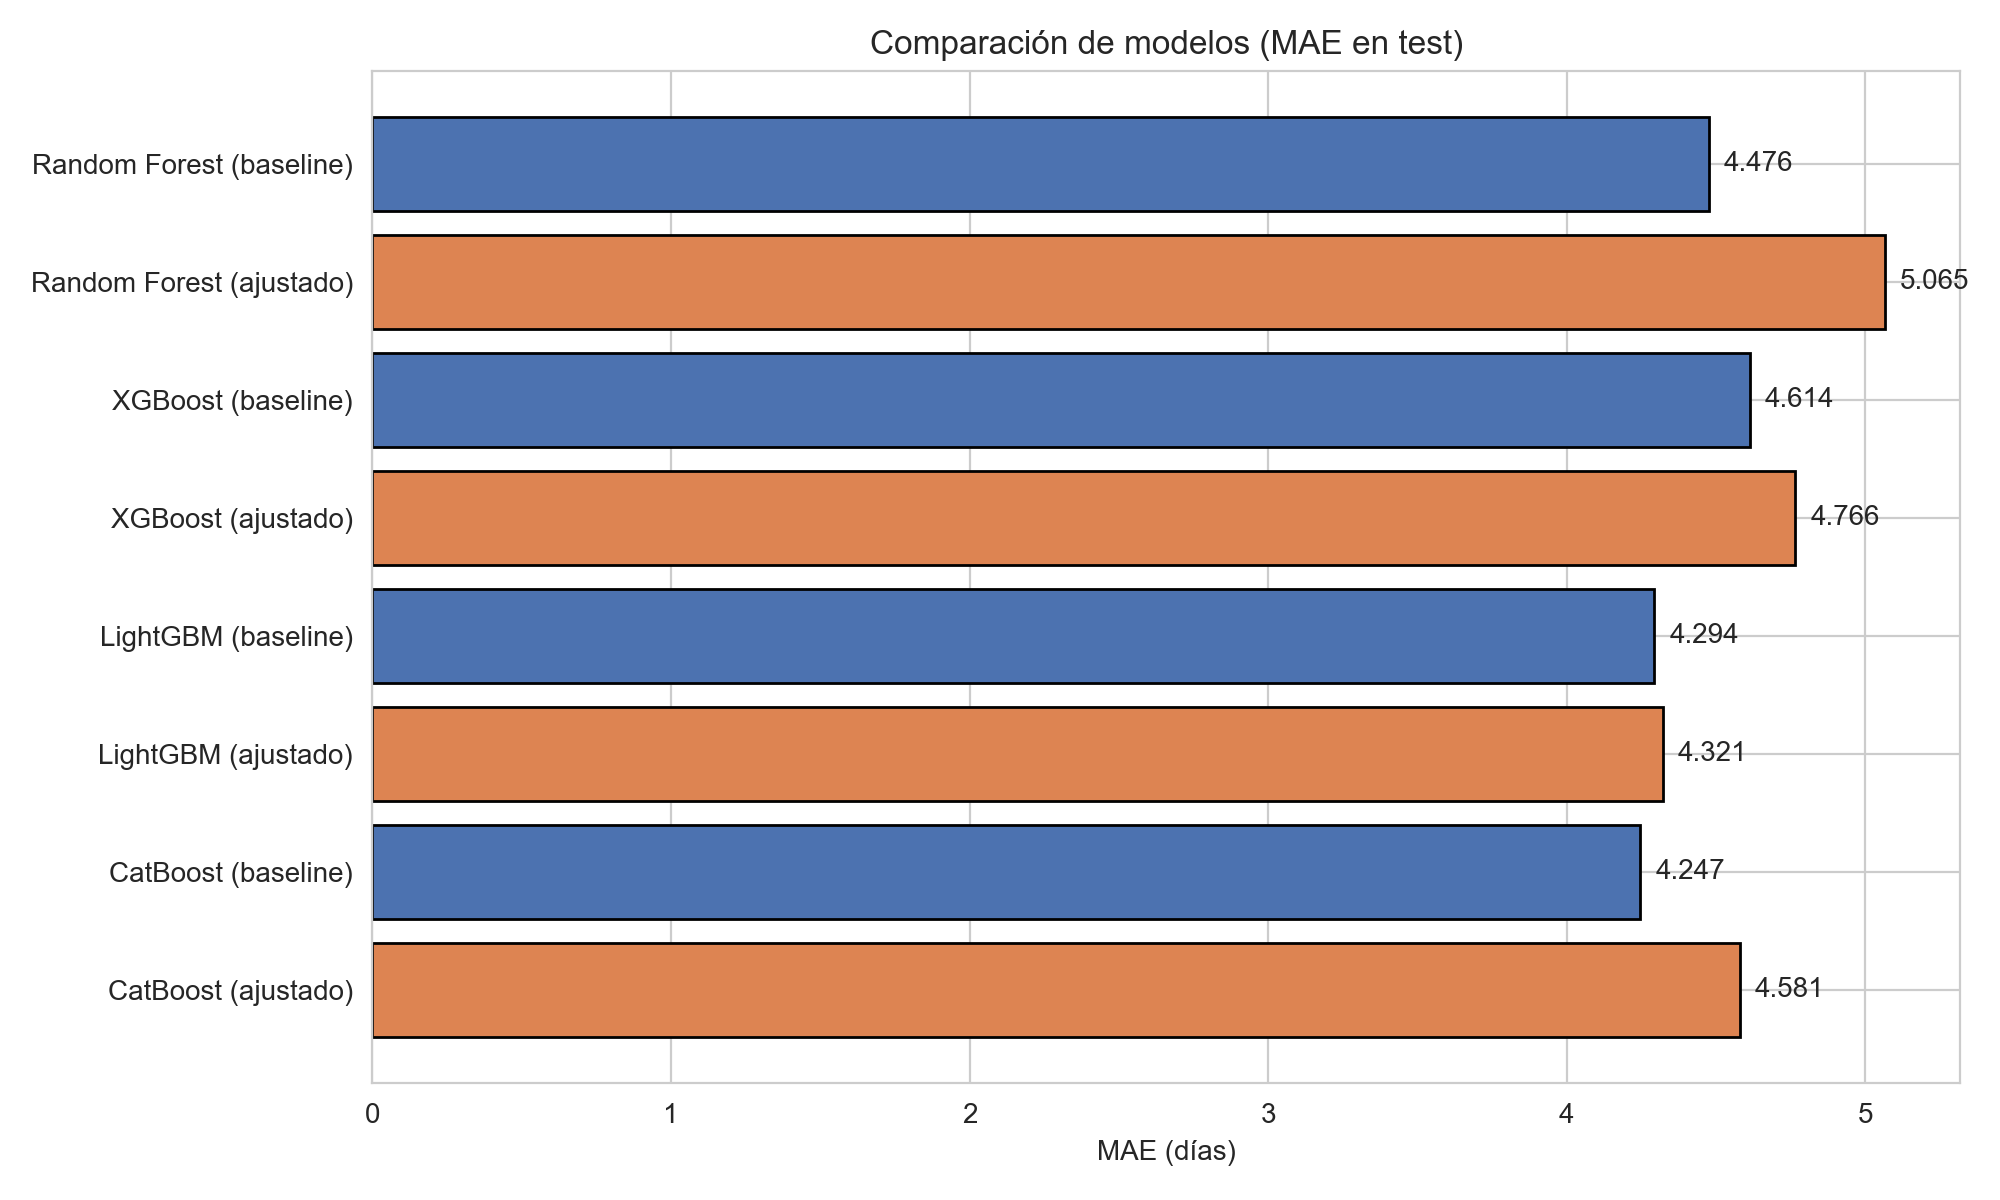
\includegraphics[width=0.95\linewidth]{figures/mae_modelos.png}
	\caption{Comparación de modelos según MAE en \textit{test}. CatBoost baseline logra el menor error; los ajustes aleatorios empeoran el desempeño.}
	\label{fig:mae_modelos}
\end{figure}
\FloatBarrier

\subsection{Importancia de predictores}

El análisis exploratorio y el desempeño de las características ingenierizadas revelan una jerarquía clara de predictores:
\begin{enumerate}
	\item \textbf{Distancia geográfica}: con correlación de 0.394, es el predictor numérico más fuerte. Cada 1000 km adicionales añaden $\sim$6.4 días al tiempo de entrega.
	\item \textbf{Ubicación regional}: los estados del norte (RR, AP, AM) promedian 26--29 días vs.\ 8--13 días en el sudeste (SP, MG, RJ), una diferencia de hasta 3$\times$. Los indicadores de cliente/vendedor remoto capturan este efecto.
	\item \textbf{Mismo estado}: las entregas intra-estatales (36\% de las órdenes) son significativamente más rápidas que las interestatales.
	\item \textbf{Características físicas}: peso, volumen y densidad muestran correlación débil con el tiempo de entrega; el factor logístico dominante es la distancia, no el tamaño del paquete.
	\item \textbf{Patrones temporales}: comprar en fin de semana o fuera de horario laboral añade menos de 0.5 días en promedio; su impacto es marginal.
\end{enumerate}
La distancia y la región explican la mayor parte de la variabilidad, mientras que las características del producto y el momento de compra tienen efecto secundario.

\section{Limitaciones}

El flujo evita fuga temporal explícita, pero persisten varias limitaciones:
\begin{itemize}
	\item Supone estabilidad logística (stock, rutas, clima); cambios abruptos pueden degradar las predicciones.
	\item No incorpora variables externas (feriados, clima, congestión), potencialmente relevantes para los valores atípicos.
	\item El sesgo negativo persistente (~-2.4 días) implica sobreestimación sistemática; requiere calibración adicional.
\end{itemize}

\section{Trabajo relacionado}

Los modelos basados en árboles han sido ampliamente usados en tabulares para predicción de tiempos y series temporales. Breiman introdujo Random Forest como ensamble robusto para manejar no linealidades sin requerir escalado de variables\cite{breiman2001random}. Chen y Guestrin popularizaron XGBoost como booster eficiente y regularizado\cite{chen2016xgboost}, base de múltiples soluciones en competiciones. LightGBM\cite{ke2017lightgbm} adoptó histogramas y crecimiento \textit{leaf-wise} para acelerar entrenamiento en columnas \textit{one-hot}, mientras que CatBoost\cite{prokhorenkova2018catboost} añadió manejo nativo de categorías y técnicas anti-\textit{leakage}. Estas familias de modelos son estándares de facto para estimar ETAs en contextos logísticos y de \textit{e-commerce}, por su buen compromiso entre precisión y costo computacional.

\section{Conclusiones y trabajo futuro}

La distancia y la ubicación regional son los factores más determinantes para estimar días de entrega en Olist. Los modelos basados en árboles capturaron este patrón sin requerir ajustes complejos. CatBoost con configuración por defecto fue el mejor equilibrio entre precisión y simplicidad, con un MAE cercano a 4.2 días y sesgo conservador.

Como trabajo futuro se propone calibrar el sesgo negativo, enriquecer el modelo con variables externas (feriados, clima o capacidad logística) y explorar modelos específicos por región para reducir la variabilidad entre estados remotos y el sudeste.

\bibliographystyle{IEEEtran}
\bibliography{references}

\end{document}
